\documentclass{article}
\usepackage{listings}
\usepackage{graphicx}

\newcommand{\SolutionName}{BinarySearch}
\newcommand{\ProjectName}{BinarySearch}

\newcommand{\code}[1]{\lstinline{#1}}

\title{GCD Static Checking Example}
\date{}


\begin{document}
\maketitle
\begin{abstract}
This example shows how to use contracts to prove some arithmetic
properties of the greatest common denominator computation.
\end{abstract}

\input{../Common/Addref.tex}

\section{Sample Walkthrough}
\label{sec:start}

After adding the proper reference, go to the Properties of project
\textsf{GCD}, select the Code Contracts pane (at the bottom), and enable static
checking by clicking on the checkbox as shown in this screenshot:
\begin{center}
  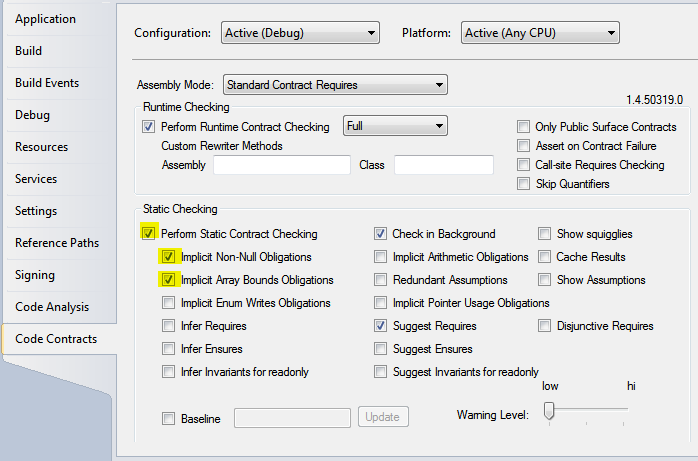
\includegraphics[width=.8\columnwidth]{ex1.png}
\end{center}

Then build the example. There should be no warnings or errors at this
point. To get static checking of arithmetic properties, such as
division by zero, we need to enable that explicitly by checking the
``Implicit Arithmetic Obligations" checkbox as shown in the following screen shot:
\begin{center}
  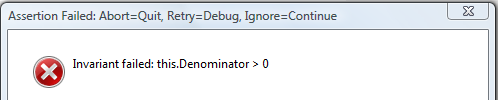
\includegraphics[width=.6\columnwidth]{ex2.png}
\end{center}
Go ahead and add this option, then build again. The warning list
should now display three warnings about possible division by zero:
\begin{center}
  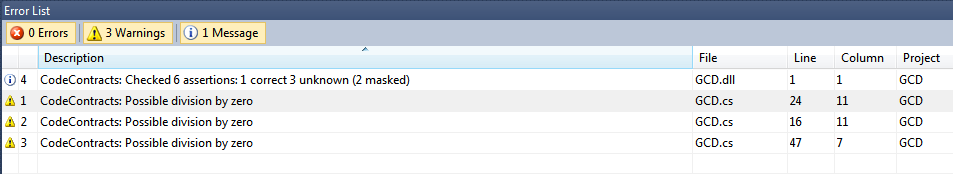
\includegraphics[width=1\columnwidth]{ex3.png}
\end{center}
Let's try to write some contracts to make sure we won't run into these
division by zero problems. Double click on the first warning. To avoid
the division by zero of the code \code{x \%= y}, we can add the
following precondition to method \code{GCD}
\begin{lstlisting}
  Contract.Requires(y > 0);
\end{lstlisting}
The second warning is about the similar division by \code{x}, so we
add a similar precondition for it:
\begin{lstlisting}
  Contract.Requires(x > 0);
\end{lstlisting}
Add those two preconditions and build again. You should now get the
following warnings:
\begin{center}
  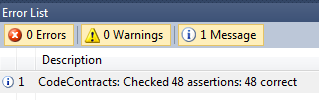
\includegraphics[width=1\columnwidth]{ex4.png}
\end{center}
The possible division by zero remaining is in the
\code{NormalizedRational} method, when dividing by the \code{gcd}
value. The \code{GCD} should never be zero, and in fact due to our
preconditions on the \code{GCD} method, our \code{GCD} will always be
positive. So let's write a postcondition on \code{GCD} that makes this
explicit. The contracts on \code{GCD} should now look as follows:
\begin{lstlisting}
public static int GCD(int x, int y)
{
  Contract.Requires(x > 0);
  Contract.Requires(y > 0);
  Contract.Ensures(Contract.Result<int>() > 0);
\end{lstlisting}
Write the \code{Ensures} and rebuild.
The checker should issue no more warnings.

%Now we are left with two
%warnings that the preconditions of the call in \code{NormalizedRational} to \code{GCD} are not
%satisfied. We can easily push these requirements onto the callers of
%this method by making them explicit preconditions of the normalized
%\code{NormalizedRational} method. In fact, the checker suggests this
%automatically, as you can see in the informational messages in the Error List.
%We can weaken the condition on \code{x}, as the code explicitly
%handles the case when \code{x} is zero. So we add the following:
%\begin{lstlisting}
%static public Rational NormalizedRational(bool pos, int x, int y)
%{
%  Contract.Requires(x >= 0);
%  Contract.Requires(y > 0);
%\end{lstlisting}
%If we build again now, the checker issues no more warnings.


\end{document}
